% ATENÇÃO - veja com o seu orientador se você vai ter este capítulo e se este vai ter nome!
\chapter{Proposta}
\label{cap:proposta}

O êxodo rural corresponde ao processo de migração em massa da população de campo para as cidades, fenômeno que costuma acontecer em períodos de tempo considerados curtos, com prazo de algumas décadas. Trata-se de um elemento diretamente associado a várias dinâmicas socioespaciais, tais como a urbanização, a industrialização, a concentração fundiária e a mecanização do campo.\cite{Pena2013}

Nos períodos de entre 1950 e 1980 o êxodo rural brasileiro chegou ao seu pico onde aproximadamente 30\% da população rural migraram para as cidades. Na ultima década, a migração perdeu velocidade, mas continuou a representar uma grande mudança no ambiente rural, onde 5,6 milhões de pessoas, 17,6\% da população rural, mudou-se para a cidade.\cite{Marra2011}

Os motivos para tal ocorrência são inúmeros, dentre eles: melhores condições de vida na cidade, o fim de unidades de produção familiares compradas por grandes latifundiários, queda na fecundidade e massiva mecanização das operações agrícolas.

Com enxada, foice e demais ferramentas, uma família não é capaz de cultivar três de acres de terra. Essa é uma das razões pelas quais tanto os agricultores familiares quanto assentados pedem veementemente para o governo para linhas de créditos a fim de se adequar a corrente de mecanização. \cite{Alves2013}

As máquinas e os equipamentos são indispensáveis para se realizarem tarefas dentro de um calendário ótimo e de acordo com as exigências de qualidade e do clima. Dão conforto aos trabalhadores e protegem sua saúde na aplicação de agrotóxicos, por exemplo. No caso de grãos, sem as plantadeiras de alta precisão, não se obtêm níveis remuneradores de produtividade. As colheitadeiras permitem realizar as tarefas num calendário compatível com as exigências dos mercados interno e externo. Na produção de leite, a ordenhadeira é fundamental para se obter nível de qualidade exigido e é importante para se obter o nível de qualidade exigido e é importante para reduzir o esforço dos trabalhadores. O Brasil dispõe de vastas áreas, dentro da fronteira agrícola já ocupada e em termos de terras degradadas, para se incorporarem à agricultura comercial. Pelos métodos manuais, tal incorporação é impossível, tanto tecnicamente como também porque grande parte da população foi drenada para as cidades. Assim a expansão da agricultura requer a mecanização.

A agricultura de precisão e uma filosofia de gerenciamento agrícola que parte de informações exatas, precisas e se completa com decisões exatas. Agricultura de precisão, também chamada de AP, é uma maneira de gerir um campo produtivo metro a metro, levando em conta o fato de que cada pedaço da fazenda tem propriedades diferentes.\cite{Tschiedel2002}

A agricultura de precisão é um sistema de manejo de produção integrado, que tenta igualar o tipo e a quantia de insumos que entram na propriedade com as necessidades da cultura em pequenas áreas dentro de um campo da propriedade. Para tal, essa filosofia anda de mão dadas com outras tecnologias: sensoriamento remoto, sistemas de informações geográficas(SIG) e de posicionamento global(GSP). A junção das tecnologias com esse tipo de pensamento pode vir a reduzir riscos nas atividades agrícolas, reduzir custo, ajudar na tomada de decisões, maior produtividade e menor impacto ambiental.
%apresentar a ideia
Com advento da mecanização agrária, da agricultura de precisão e da constante diminuição da população rural, consequentemente, da mão de obra, a automação do campo vem como ideia plausível e factível de como resolver e incorporar tais aspectos nos próximos anos na já industrializada produção do campo. Tendo em vista os vários frontes de pesquisa na área da automação agrária, é concebível a criação de um veículo autônomo terrestre que possa exercer certas funções no campo sem a interferência humana. 

Para tal, é necessário um algoritmo robusto, capaz de interpretar os dados dos sensores, bem como dados do GPS, combinando-os com mapas georreferenciados para que possa traçar um caminho seguro, seja ele de translado ou mesmo durante as tarefas no campo \ref{fig:entrada:saida}. O algoritmo deve ser capaz de, mediante obstáculos, recalcular sua rota, evitando o obstáculo e continuar seu trabalho, evitando danos ao próprio veiculo, a outros veículos ou até mesmo pessoas. Em adição, o algoritmo deve ser capaz de saber sua localização em relação a área de operação, tomando decisões de como atingi-la com certo nível de precisão. Em relação a área e operação, o veículo deve ser capaz de navegar por toda a área sem passar pelo mesmo caminho, evitando desperdício de recursos e de tempo.

\begin{figure}[H]
    \centering
    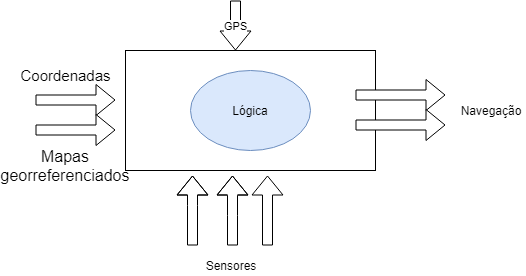
\includegraphics[width=0.75\textwidth]{figuras/entradaSaida.png}
    \caption{Conceito do algoritmo}
    \label{fig:entrada:saida}
\end{figure}

O algoritmo deve, de forma constante, medir a distância entre o seu ponto de destino e sua posição atual, ao mesmo tempo em que verifica sua atual direção e compara com a direção do ponto de destino. Em paralelo a isso, os sensores de distância devem ser lidos ininterruptamente em busca de possíveis obstáculos, evitando possíveis colisões. 
\begin{figure}[H]
    \begin{center}
    % jacto
        \subfigure[]{
            \label{fig:distância:alvo}
            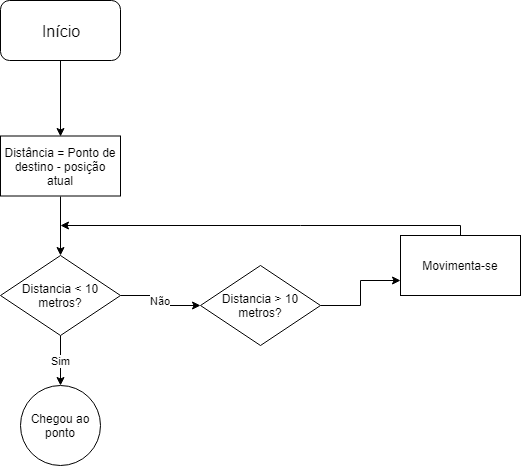
\includegraphics[width=0.4\textwidth]{figuras/ManicaDeEstados.png}
        }
        % new holland
        \subfigure[]{
            \label{fig:obstaculos}
            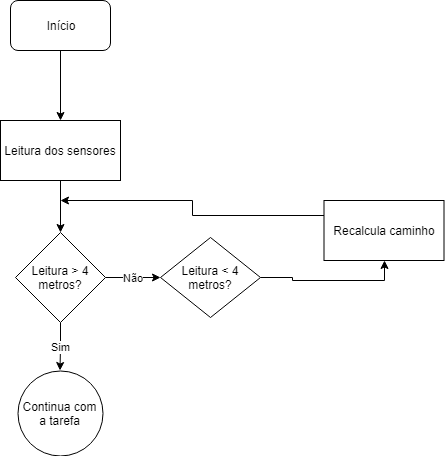
\includegraphics[width=0.4\textwidth]{figuras/obstaculos.png}
        }
      
    \end{center}
    \caption{%
        (a) Distância entre os pontos, (b)Evitar os obstáculos
     }%
\end{figure}



A ideia da criação de um veículo dessa categoria une a mecanização com a agricultura de precisão, tendo em vista a união dos dois mundos na criação de um equipamento que possa, através de sensores, compreender o ambiente ao seu redor, bem como combinar dados provenientes de GPSs para que se situe dentro de uma área pré-estabelecida e possa, com segurança, exercer suas funções durantes horas, quiçá dias, dadas boas condições de operação. O Brasil é um país de dimensões continentais do clima variando entre o equatorial até o semiárido com grande incidência de raios solares e combinando isso ao ambiente de operação, a utilização de fontes de energia provenientes da luz solar se torna interessante e implementável.

Em essência a utilização de sistemas fotovoltaicos, combinados a algoritmos de melhor caminho, sensores de distância, GPSs e um sistema de monitoramento que possa acompanhar o desempenho do veículo no campo, assim como em \textbf{4.3}, pode vir a culminar em um veículo terrestre de médio porte capaz de pulverizar, semear ou coletar informações sobre o campo.

A proposta a ser descrita idealiza um veículo de 4 rodas, movido por um único motor elétrico, sensores de ultrassônicos de distância, GPS e luzes, bem como painéis fotovoltaicos para produção de energia. A utilização de lagartas mecânicas foi descartada dada a complexidade da manutenção, a possibilidade de durante uma curva, uma das lagartas sair dos trilhos causando danos a suspensão e imobilizando o veiculo, bem como os danos causados ao solo. 

A figura \ref{fig:sketchup:vaa} apresenta uma visão geral do veículo, onde observa-se a maioria dos componentes externos: GPS, painel fotovoltaico e os sensores ultrassônicos. Logo abaixo do apoio superior, ficaram os demais componentes, tais como Arduinos, Pontes H, o \textit{shield} do GPS e outros servos. 
\begin{figure}[H]
    \centering
    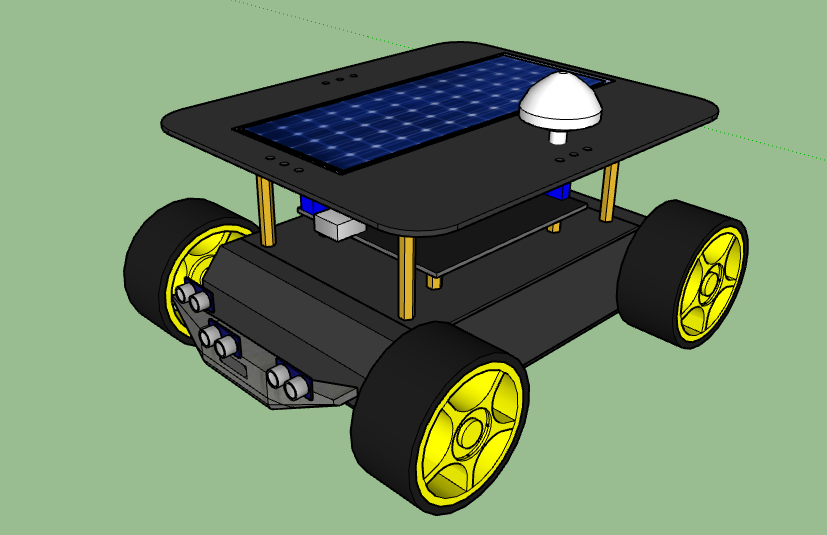
\includegraphics[width=0.75\textwidth]{figuras/chassi_vaa_completo.png}
    \caption{Esquema do chassi feito no Sketchup}
    \label{fig:sketchup:vaa}
\end{figure}
O veículo apresentado na figura \ref{fig:sketchup:vaa} sofrerá revisões ao longo do trabalho, principalmente em relação ao seu chassi, dado a necessidade de uma altura maior e espaço entre rodas. Contudo, a parte superior deve continuar nesse \textit{layout}.
O veículo possuirá, inicialmente, 3 sensores ultrassônicos dispostos na frente do mesmo, afim de captar possíveis obstáculos em sua rota, fazendo com o veiculo seja capaz de realizar manobras para evitar colisões e manter-se em distância segura das plantas do campo. Na figura \ref{fig:ultrasonico:vaa} podemos observar o esquemático gerado no Fritzing\footnote{http://fritzing.org/home/} representando um Arduino UNO R3 e 3 sensores ultrassônicos HCSR05.
\begin{figure}[H]
    \centering
    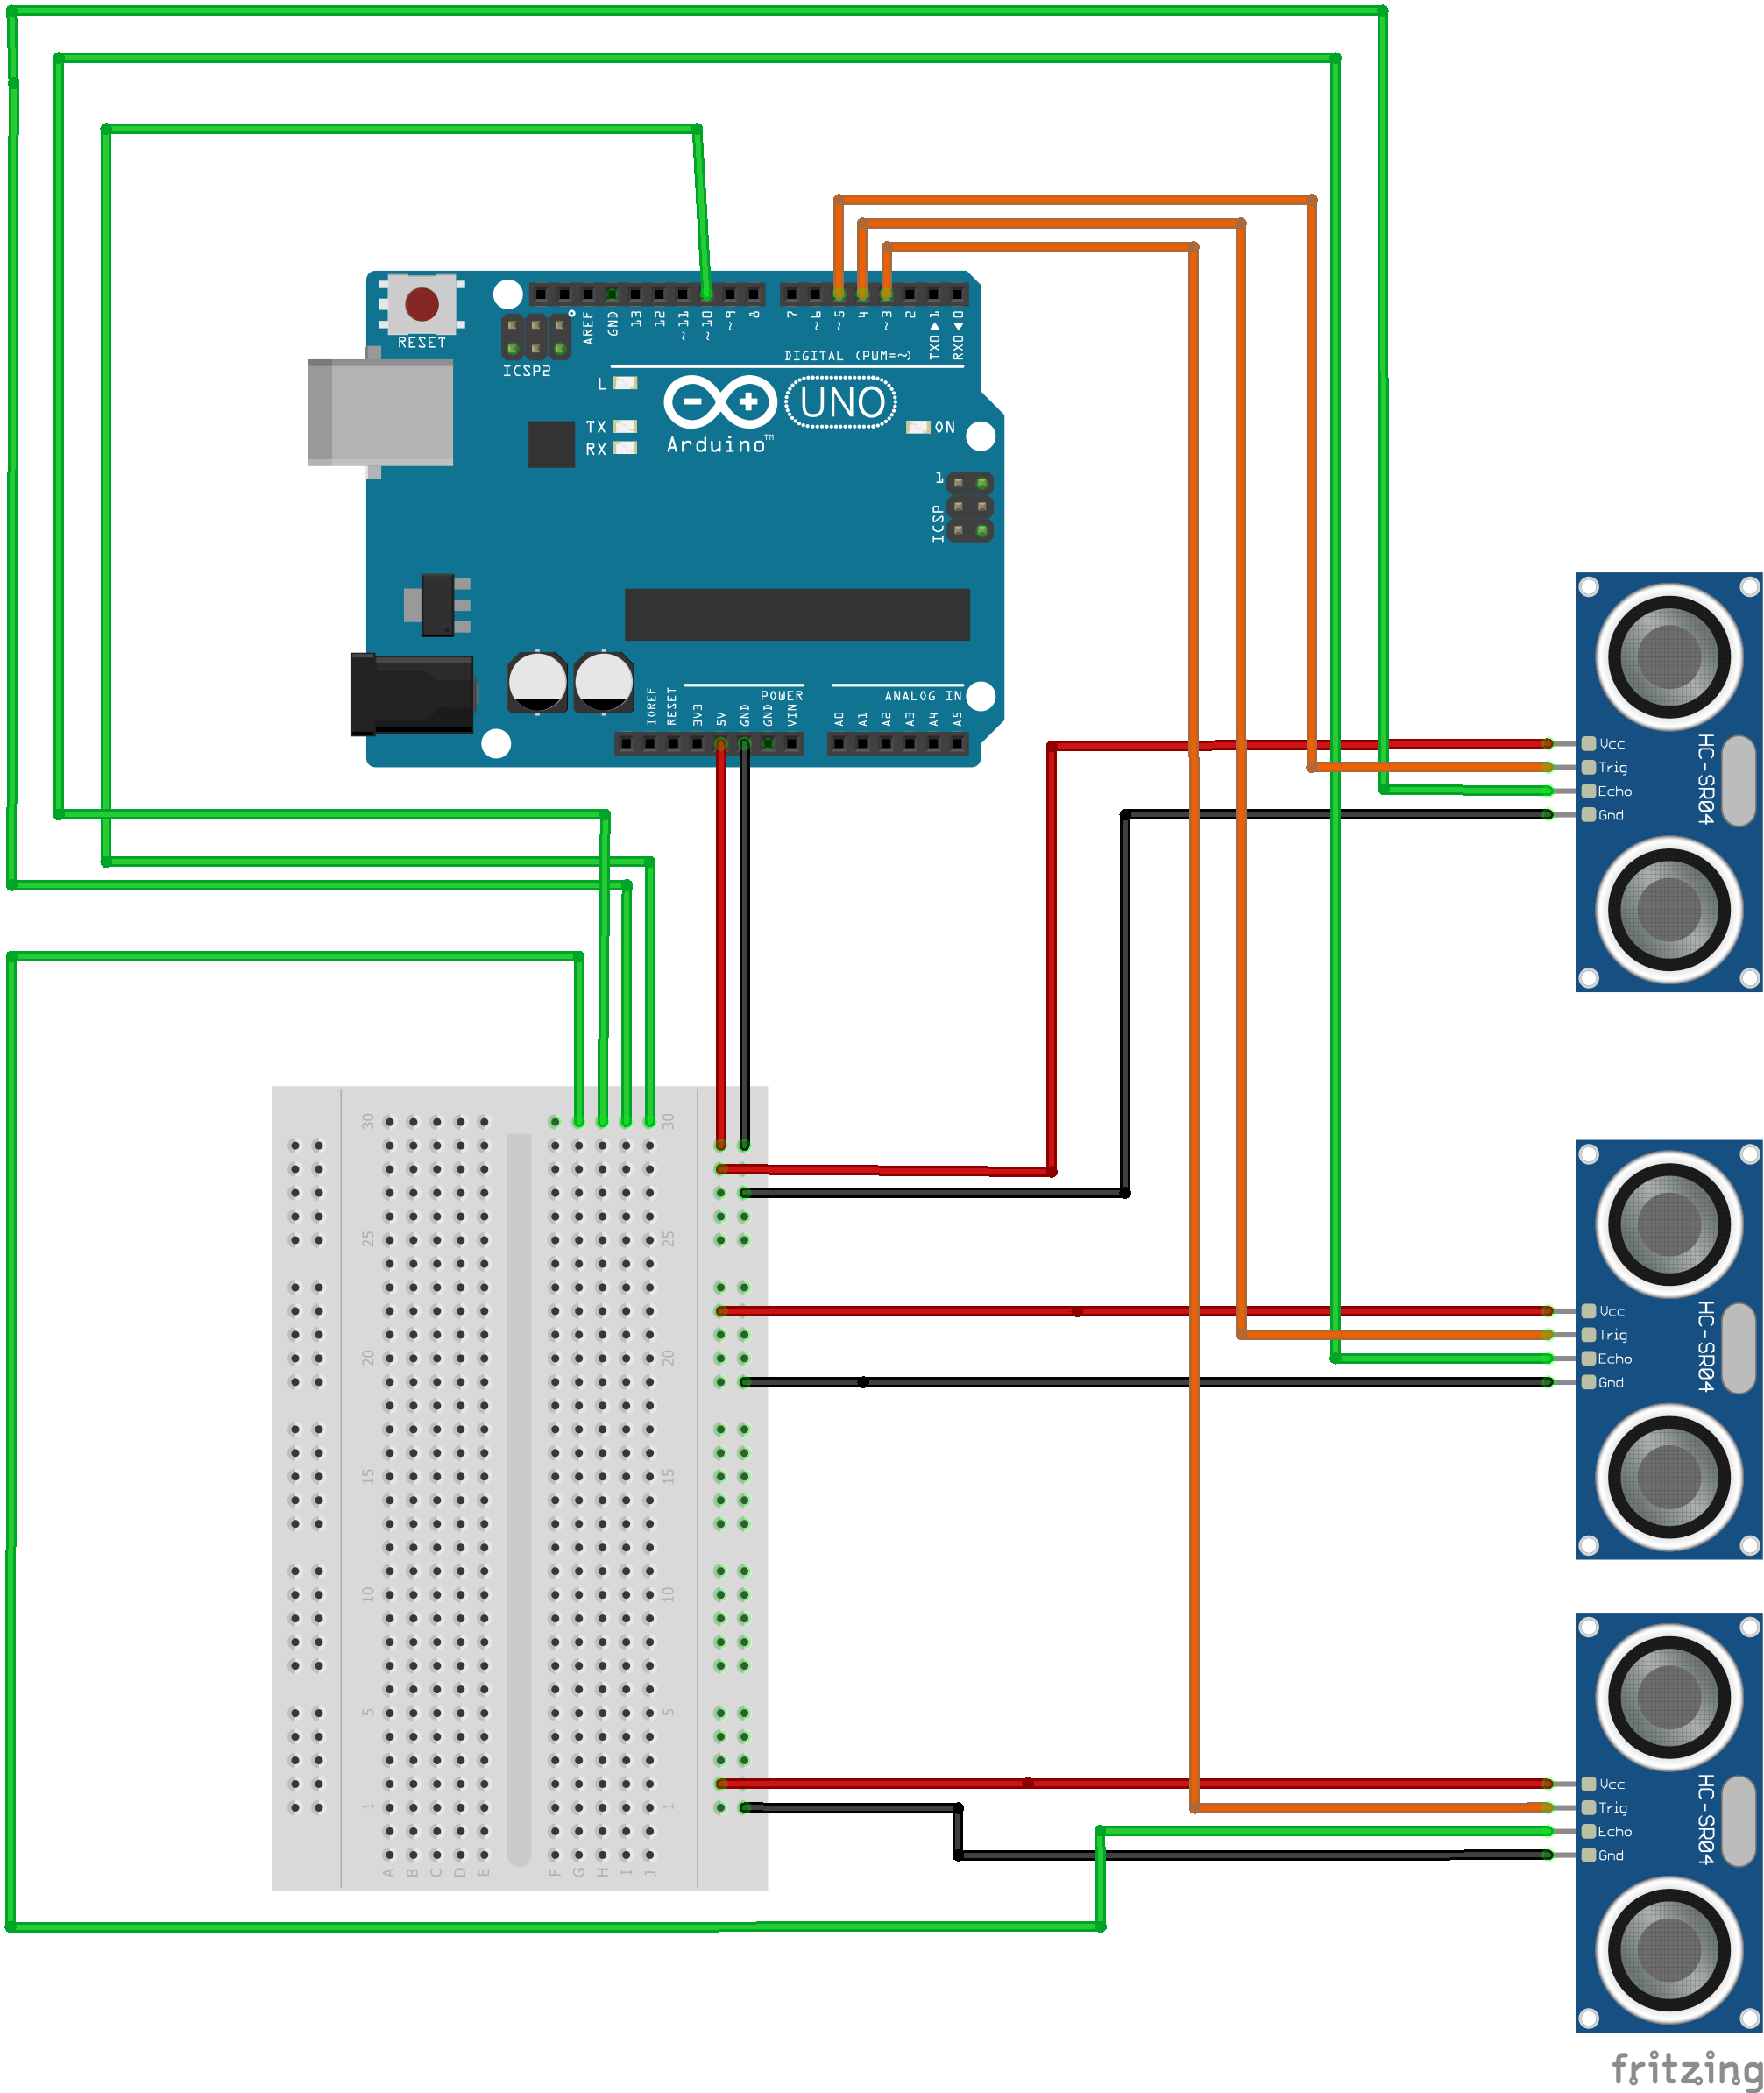
\includegraphics[width=0.5\textwidth]{figuras/ultrassonico_bb.png}
    \caption{Esquemático dos sensores ultrassônicos gerado no Fritzing utilizando componentes disponíveis}
    \label{fig:ultrasonico:vaa}
\end{figure}

O módulo GPS a ser usado será o GSM GPRS SIM808 em forma de\textit{ shield} que será acoplado diretamente ao Arduino, ilustrado na figura \ref{fig:gps:vaa}.
\begin{figure}[H]
    \centering
    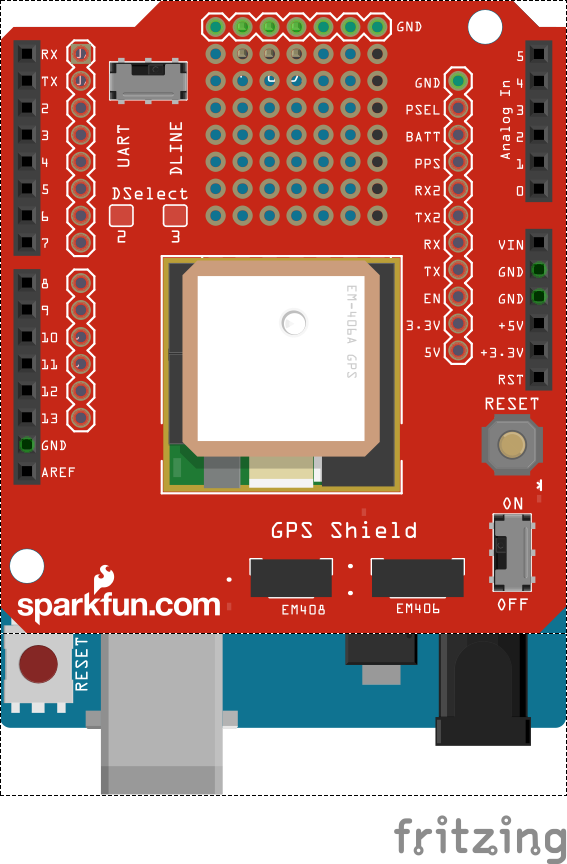
\includegraphics[width=0.4\textwidth]{figuras/arduinoGPS_bb.png}
    \caption{Shield GPS acoplado a um Arduino UNO R3}
    \label{fig:gps:vaa}
\end{figure}


/***DESCREVER***/

\begin{figure}[H]
    \centering
    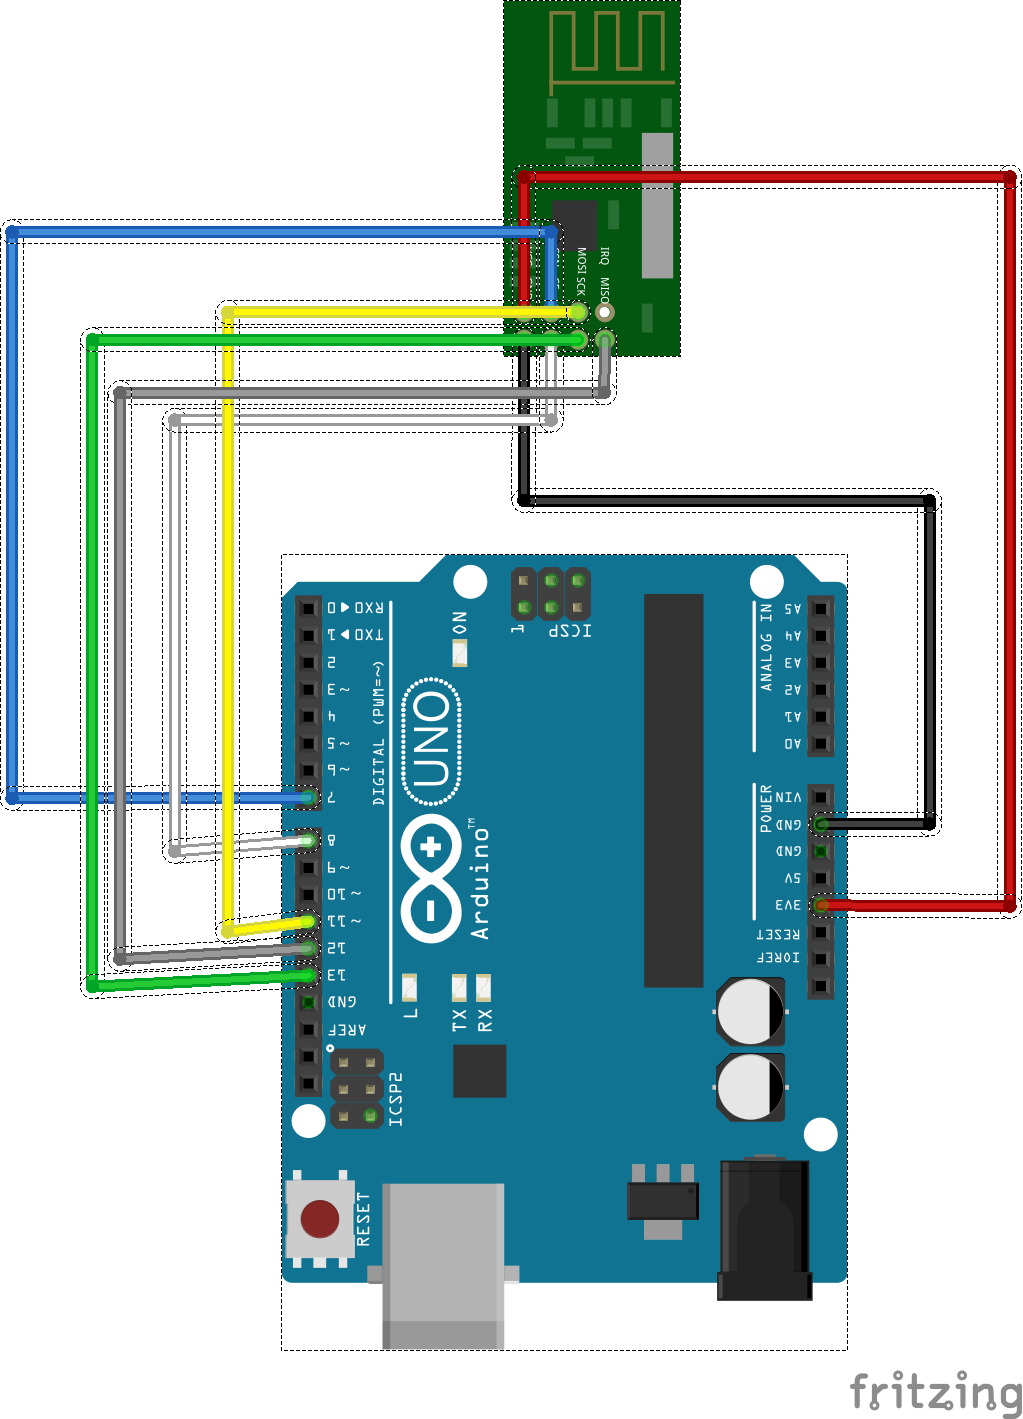
\includegraphics[width=0.5\textwidth]{figuras/radio_bb.png}
    \caption{Esquema do chassi}
    \label{fig:sketchup:vaa}
\end{figure}

\begin{figure}[H]
    \centering
    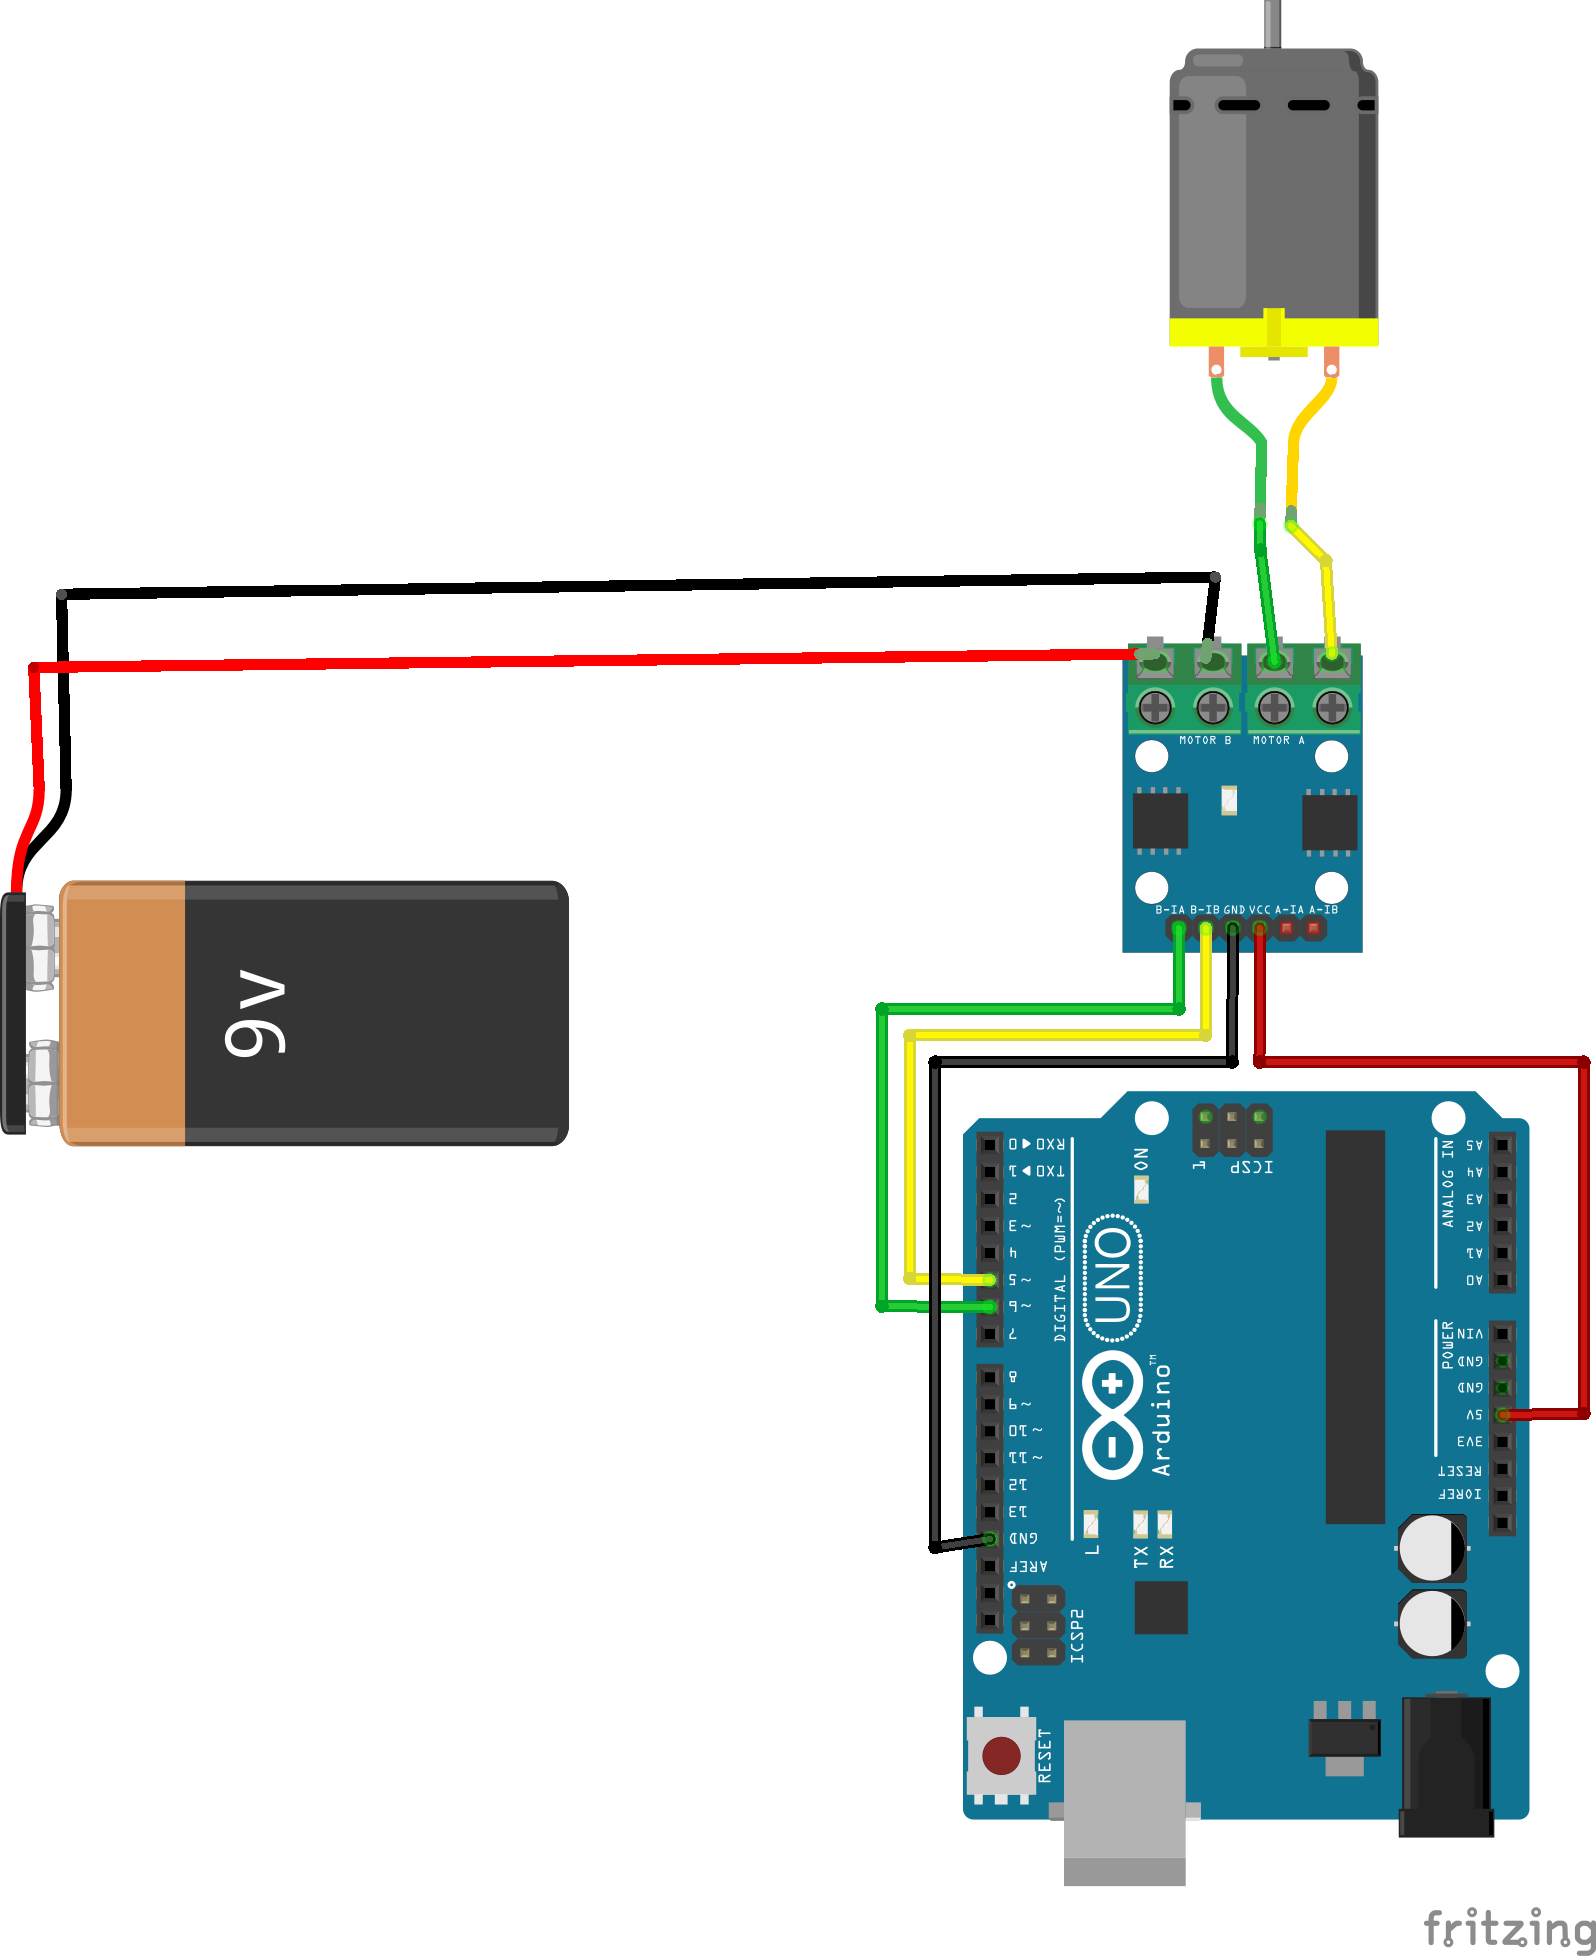
\includegraphics[width=0.5\textwidth]{figuras/motor_bb.png}
    \caption{Esquema do chassi}
    \label{fig:sketchup:vaa}
\end{figure}

A fim de operar esse veículo durante horas, será necessário criar um sistema fotovoltaico capaz de alimentar os componentes, bem como armazenar energia em baterias para que o mesmo continue operando mesmo em condições de baixa luminosidade ou até mesmo durante a noite. Para tal, devemos obter as especificações quanto ao consumo elétrico de cada componente, a fim de calcular qual o gasto, a autonomia do sistema, bem como os demais componentes a serem utilizados.

De inicio, deve-se quantificar, bem como obter os dados de todos os componentes do sistema, os quais estão presentes na tabela \ref{cap:proposta:tab:quantificar}:

%https://www.tablesgenerator.com/#

\begin{table}[]
\centering
\caption{Consumo por 8 horas de uso}
\label{cap:proposta:tab:quantificar}
\begin{tabular}{lll|l|l|}
\hline
\multicolumn{1}{|l|}{\textbf{Quantidade}} & \multicolumn{1}{l|}{\textbf{Descrição}}   & \textbf{Potência} & \textbf{Tempo de Uso} & \textbf{Consumo} \\ \hline
\multicolumn{1}{|l|}{6}                   & \multicolumn{1}{l|}{Arduino UNO R3}       & 0,54W             & 8 horas               & 4,32W            \\ \hline
\multicolumn{1}{|l|}{2}                   & \multicolumn{1}{l|}{Raspberry Pi}         & 1,2               & 8                     & 9,6W             \\ \hline
\multicolumn{1}{|l|}{1}                   & \multicolumn{1}{l|}{Motor elétrico 1/4hp} & 127w             & 8                     & 1016         \\ \hline
\multicolumn{1}{|l|}{1}                   & \multicolumn{1}{l|}{Motor elétrico}       & 30w               & 8                     & 240w             \\ \hline
\multicolumn{1}{|l|}{1}                   & \multicolumn{1}{l|}{NRF24L01}             & 0,115W            & 8                     & 0,92w            \\ \hline
\multicolumn{1}{|l|}{3}                   & \multicolumn{1}{l|}{HC-SR04}              & 0,015             & 8                     & 0,12w            \\ \hline
\multicolumn{1}{|l|}{1}                   & \multicolumn{1}{l|}{GPS shield}           & 0,02w             & 8                     & 0,16w            \\ \hline
                                          &                                           &                   & \textbf{Total}        & 1271,12w      \\ \cline{4-5} 
\end{tabular}
\end{table}

Na tabela acima obtemos o consumo total de todos os componentes durante um período de 8 horas. A escolha o Inversor de Corrente Autônomo deve obedecer a uma faixa de potência continua entre 226,98W e 317,78W, baseando-se no calculo feito a partir da potencia instantânea, vista na tabela \ref{cap:proposta:tab:instantaneo}: 

\begin{table}[]
\centering
\caption{Consumo instantâneo}
\label{cap:proposta:tab:instantaneo}
\begin{tabular}{l|l|l|}
\hline
\multicolumn{1}{|l|}{\textbf{Quantidade}} & \textbf{Descrição}   & \textbf{Potência} \\ \hline
\multicolumn{1}{|l|}{6}                   & Arduino UNO R3       & 0,54W             \\ \hline
\multicolumn{1}{|l|}{2}                   & Raspberry Pi         & 1,2               \\ \hline
\multicolumn{1}{|l|}{1}                   & Motor elétrico 1/4hp & 127w             \\ \hline
\multicolumn{1}{|l|}{1}                   & Motor elétrico       & 30w               \\ \hline
\multicolumn{1}{|l|}{1}                   & NRF24L01             & 0,115W            \\ \hline
\multicolumn{1}{|l|}{3}                   & HC-SR04              & 0,015             \\ \hline
\multicolumn{1}{|l|}{1}                   & GPS shield           & 0,02w             \\ \hline
                                          & \textbf{Total:}      & 158,89        \\ \cline{2-3} 
\end{tabular}
\end{table}
Onde, calculamos:
\[F_{max}=317,78w\] e \[F_{min}=226,98w\]
Referentes à faixa de operação com folga para o inversor autônomo. 

A seguir, calculamos o valor da energia gerada pelo sistema, dada uma eficiência máxima do inversor autônomo de 90\%, bem como a sua tensão de 24V:
\[ED =\frac{Consumo Diário}{Eficiência Máxima}\]
\[ED = \frac{1271,12}{0,9}\]
\[ED = 1412,35\]
Com isso, podemos calcular a energia real da instalação, sendo:
\[ER=\frac{ED}{R}\]
\[ER=\frac{1412,35}{0,89}\]
\[ER=1587\]

Para realizarmos os cálculos, assumimos os valores hipotéticos a uma bateria com as seguintes características apresentadas na tabela \ref{cap:proposta:tab:bateria}:
\begin{table}[h]
\centering
\caption{Bateria hipotética}
\label{cap:proposta:tab:bateria}
\begin{tabular}{|l|l|}
\hline
\multicolumn{2}{|c|}{\textbf{Bateria Hipotética}} \\ \hline
\textbf{Capacidade Real}          & 210Ah         \\ \hline
\textbf{Vb}                       & 12V           \\ \hline
\textbf{CN}                       & 105Ah         \\ \hline
\textbf{Pd}                       & 0,6           \\ \hline
\end{tabular}
\end{table}

Por fim, calcula-se o valor da capacidade útil do banco de baterias, assumindo que N terá o valor de $\frac{1}{24}$*8, adaptando a formula a consumo por horas. Temos que:
\[CU=\frac{ER*N}{Vi}\]
\[CU=\frac{1587*0,333}{24}\]
\[CU=22,03\]
Atentando-se de que as baterias não podem ser descarregadas em sua totalidade, calcula-se a carga real:
\[CR=\frac{CU}{PD}\]
\[CR=\frac{22,03}{0,6}\]
\[CR=36,71Ah\]
Finalmente, calcula-se o numero de baterias a serem utilizadas pelo sistema, tanto em série como em paralelo:
\[NB=\left ( \frac{CR}{CN} \right )*\left ( \frac{Vi}{VB} \right )\]
\[NB=\left ( \frac{36,71}{105} \right )*\left ( \frac{24}{12} \right )\]
\[NB=0,699\]
Como o resultado mostra, uma bateria será o suficiente para todo o sistema, e segundo os cálculos, com sobra.

